\subsection{Loop antenna}\label{sec:loop_sim}
\subsubsection{Setup}

\FloatBarrier

\begin{figure}[tbp]
	\centering
	\raisebox{-4.5mm}{
	\begin{subfigure}[t]{0.49\textwidth}
		\centering
		\includegraphics[width=1\linewidth]{content/img/loop_near_field}
		\caption{Electric near-field intensity of loop antenna}
		\label{fig:loopnearfield}
	\end{subfigure}
}
	\hfill
	\begin{subfigure}[t]{0.48\textwidth}
		\centering
		\includegraphics[width=1\linewidth]{content/img/loop_antenna}
		\caption{Geometry of loop antenna}
		\label{fig:loopantennageometry}
	\end{subfigure}
	
	\caption{The geometry of the loop antenna assimilates a square with round edges. The height and width of the antenna equal $h=w=1.6$\,mm. The return path leads back to the PEC surface of the TEM cell. The electric near-field shows a large displacement current and voltage drop near the feed-point.}
	\label{fig:loopantenna}
\end{figure}

In contrast to the monopole antenna, the loop antenna is the most fundamental antenna capable of generating a magnetic dipole moment and is therefore selected as the second case for further analysis. The geometry of the loop antenna model, positioned inside the TEM cell and connected to a feedpoint on the top cell wall, is shown in \autoref{fig:loopantennageometry}. The antenna consists of three wire segments, each of length $h = w = 1.6\,$mm, and the PEC surface as return path, yielding a total circumference of $C = 6.4\,$mm. The antenna remains electrically short ($C < \lambda/10$) for frequencies up to $4.69\,$GHz. A square loop is preferred over a round geometry in the numerical model, as it enables more accurate mesh generation and cleaner interpretation of the resulting equivalent dipole moments. The mesh is refined on the antenna surface and near the feedpoint, following the preliminary discussion in \cref{sec:mesh}.

The loop antenna is oriented such that the normal vector of its enclosed surface is aligned with the $x$-direction, which maximizes the coupling with the magnetic field component of the TEM mode. Unlike the monopole antenna discussed in \cref{sec:monopole}, the loop antenna provides a current return path. The circulating current induces a rotational electric field, equivalent to a net magnetic field intensity through the loop area, thereby giving rise to a magnetic dipole moment as described by \eqref{eqn:mag_dipole_moment_tem}. Furthermore, displacement currents between the antenna and the septum contribute an electric dipole moment, as expressed in \eqref{eqn:me_i}, analogous to the behavior observed for the monopole antenna. The resulting equivalent electric and magnetic dipole moments are analyzed in detail in \cref{sec:eq_dip_loop}.

The output power produced by the equivalent dipole moments is compared to that radiated by the loop antenna in \cref{sec:output_power_loop}, validating the equivalent dipole models. In \cref{sec:geom_dip_loop}, the influence of the loop antenna geometry is examined by varying its height and width, and analyzing the resulting equivalent dipole moments. This parametric study provides additional insight into how the geometrical properties of the loop antenna influence the equivalent dipole moments.

The electric and magnetic coupling mechanisms between the loop antenna and the TEM cell are directly reflected in the frequency-dependent behavior of the feed voltage, feed current, and antenna impedance. As the relationship between these quantities governs the overall coupling behavior, it is analyzed in \cref{sec:loop_electrical_characteristics}. In addition, the current distribution induced on the septum for varying antenna placements and frequencies is investigated in \cref{sec:current_dist_septum_loop}, with particular attention to the influence of the propagating TEM and TE\textsubscript{01} modes on the coupling behavior.

Following the approach established for the monopole antenna, the theoretical framework and numerical results are combined to derive an equivalent circuit model, presented in \cref{sec:eqc_loop}. This equivalent circuit provides deeper insight into the coupling mechanisms between the antenna and the TEM cell, as well as the interplay between the generated electric and magnetic dipole moments.

\subsubsection{Equivalent dipole moments}\label{sec:eq_dip_loop}

The equivalent dipole moments of the loop antenna are numerically derived by applying \eqref{eqn:ifa_me} and \eqref{eqn:ifa_mm}, and are presented as a function of frequency in \autoref{fig:dipole_moments_loop_antenna}. The phases of the output port powers at ports 1 and 2 are shown in \autoref{fig:loopphase}. Unlike the monopole antenna case, where the phase shift remained zero across the entire investigated frequency range, this phase information is essential for the decomposition of the equivalent dipole moments. A phase shift of zero between the output port powers indicates the presence of an electric dipole moment, whereas a phase shift of $\pm\pi$ is characteristic of a magnetic dipole moment. A phase shift between $0$ and $\pi$ indicates a superposition of both dipole moment contributions, as discussed in detail in \cref{sec:equ-dip-mom}.

The phase shift approaches $\pi$ at low frequencies, indicating that the magnetic dipole moment $\mathbf{m}_m$ dominates over the electric dipole moment $\mathbf{m}_e$. However, the phase shift decreases with frequency, raising the electric dipole moment as a consequence. In contrast to the monopole antenna, $\mathbf{m}_e$ and $\mathbf{m}_m$ thereby demonstrate non-linear behavior over frequency.

\begin{figure}[tbp]
	\centering
	\begin{subfigure}[t]{0.5\textwidth}
		\centering
		\includegraphics[width=1\linewidth]{content/img/dipole_moments_loop_antenna.png}
		\caption{Equivalent dipole moments}
		\label{fig:dipole_moments_loop_antenna}
	\end{subfigure}
	\hfill
	\begin{subfigure}[t]{0.48\textwidth}
		\centering
		\includegraphics[width=1\linewidth]{content/img/loop_phase}
		\caption{Phase of the power at each output port}
		\label{fig:loopphase}
	\end{subfigure}
	
	\caption{Equivalent electric and magnetic dipole moments of the loop antenna as a function of frequency, and the related phase of the power at each output port}
	\label{fig:moments-phase-loop}
\end{figure}

%The surface of the loop equals $S=1.68\,\mathrm{mm}^2$. The magnetic dipole moment $\mathbf{m}_m$ can be approximated by applying \crefrange{eqn:e_a_closed_int}{eqn:m_v}, using the normalized magnetic field intensity of the TEM mode $\mathbf{h}_\mathrm{TEM}^\pm$ and the feed voltage in \autoref{fig:loopfeedreturncurrent}. At 3\,GHz, for example, this yields
%
%\begin{equation}
%	\mathbf{m}_m (f=3\,\mathrm{GHz})=I()\cdot j\omega \mu_0 \frac{S\cdot(\mathbf{h}^-_\mathrm{TEM} - \mathbf{h}^+_\mathrm{TEM})}{2\mathbf{e}^\pm_\mathrm{TEM}\cdot k_0}
%\end{equation}

\subsubsection{Output power}\label{sec:output_power_loop}

The output power and the electric field intensity $E^\pm_y$ at $x=0$, $y=b/4$, $z=\pm l/2$ induced by the loop antenna at the output ports are shown in \autoref{fig:loopopower}. In comparison to the monopole antenna results presented in \autoref{fig:monopoleoutputpower}, both quantities increase more slowly with frequency. This is directly attributed to the concave frequency dependence of the magnetic dipole moment $\mathbf{m}_m$, given that the output power scales quadratically with the dipole moment amplitude. The increase in $\mathbf{m}_e$ does not compensate for this power reduction, as its influence on the output power is small, demonstrated by the analysis in \cref{sec:geom_dip_loop}. The investigation demonstrates that the increasing capacitive coupling at higher frequencies enhances the electric dipole moment contribution and partially opposes the magnetic dipole moment, thereby reducing the overall power transfer.

\autoref{fig:loopopowercomp} demonstrates the output power generated by the equivalent dipole moments $\mathbf{m}_m$, $\mathbf{m}_e$ and the loop antenna. The values agree within $\pm10\,$µW, thereby supporting the validity of the dipole moment model.

\begin{figure}[tbp]
	\centering
	\begin{subfigure}[b]{0.48\textwidth}
		\centering
		\includegraphics[width=1\linewidth]{content/img/loop_opower}
		\caption{Electric field and output power}
		\label{fig:loopopower}
	\end{subfigure}
	\hfill
	\begin{subfigure}[b]{0.5\textwidth}
		\centering
		\includegraphics[width=1\linewidth]{content/img/loop_opower_comp}
		\caption{Comparison of output powers}
		\label{fig:loopopowercomp}
	\end{subfigure}
	
	\caption{Electric field in y-direction $E_\mathrm{y}$ at $x=0, y=b/4, z=\pm l/2$, and the closely related power at one of the output ports, derived with the S-parameters in \autoref{eqn:power_antenna}. The output power produced by the loop antenna is compared with that generated by the equivalent dipole moments.}
	\label{fig:looppowercomparisons}
\end{figure}

\subsubsection{Electric and magnetic energy}

The electric and magnetic energy stored in the TEM cell and produced by the loop antenna are shown in \autoref{fig:loopelectromagneticenergy}, derived by computing \eqref{eqn:em_energy} over the TEM cell volume. At low frequencies, the loop antenna predominantly generates magnetic energy, consistent with its dominant magnetic dipole moment. However, with increasing frequency, the electric energy stored in the TEM cell grows rapidly, associated with increasing electric field intensities. This behavior can be directly connected to the increasing electric dipole moment of the loop antenna, which is driven by the growing displacement currents associated with the rising electric field intensity between the antenna and the septum.

\begin{figure}[htbp]
	\centering
	\includegraphics[width=1\linewidth]{content/img/loop_electromagnetic_energy}
	\caption{Electric and magnetic energy stored in the TEM cell as a function of frequency, produced by the loop antenna.}
	\label{fig:loopelectromagneticenergy}
\end{figure}

\subsubsection{Influence of geometry on dipole moments}\label{sec:geom_dip_loop}

The influence of the antenna geometry on the coupling behavior is investigated to explain the role of geometrical parameters in determining the equivalent dipole moments. The height $h$ and width $w$ of the loop antenna are systematically varied, and the resulting dipole moments and input power consumption are compared.

\begin{figure}[htbp]
	\centering
	\begin{subfigure}[t]{0.5\textwidth}
		\centering
		\includegraphics[width=1\linewidth]{content/img/loop-geomg-comp}
		\caption{Equivalent dipole moments}
		\label{fig:loop-geomg-comp}
	\end{subfigure}
	\hfill
	\begin{subfigure}[t]{0.48\textwidth}
		\centering
		\includegraphics[width=1\linewidth]{content/img/loop-geom-power}
		\caption{Output power}
		\label{fig:loop-geom-power}
	\end{subfigure}
	
	\caption{Equivalent dipole moments and output power for two loop antenna configurations: $h=2.16\,\mathrm{mm},\, w=1.4\,\mathrm{mm}$ and $h=1.2\,\mathrm{mm},\, w=2.36\,\mathrm{mm}$. The electric dipole moment $\mathbf{m}_e$ is weighted by $\eta_0$ to enable direct comparison with $\mathbf{m}_m$.}
	\label{fig:loop-geom-sweep}
\end{figure}

Both configurations share an identical loop area, and consequently exhibit the same magnetic dipole moment $\mathbf{m}_m$, in agreement with \eqref{eqn:e_a_closed_int} and \eqref{eqn:e_b_closed_int}. The nonlinear frequency dependence of $\mathbf{m}_m$ persists across both configurations. In contrast, the electric dipole moment $\mathbf{m}_e$ exhibits a strong dependence on the antenna height $h$. As depicted in \autoref{fig:loop-geomg-comp}, the configuration with $h = 2.16\,\mathrm{mm}$ generates an electric dipole moment more than twice that of the configuration with $h = 1.2\,\mathrm{mm}$, which is a direct consequence of the increased displacement currents arising from the reduced distance between the antenna and the septum. This result is consistent with \eqref{eqn:me_i}, which relates the displacement current between the antenna conductor and the septum to $\mathbf{m}_e$.

Finally, as shown in \autoref{fig:loop-geom-power}, the configuration producing the larger electric dipole moment also yields a slightly higher output power, although the difference remains small. This demonstrates the comparatively limited influence of $\mathbf{m}_e$ on the output power relative to $\mathbf{m}_m$. 


\subsubsection{Feed voltage, current and impedance}\label{sec:loop_electrical_characteristics}


\begin{figure}[tbp]
	\centering
	\begin{subfigure}[t]{0.45\textwidth}
		\centering
		\includegraphics[width=1\linewidth]{content/img/loop_feed_return_current_voltage}
		\caption{Voltage and current}
		\label{fig:loopfeedreturncurrent}
	\end{subfigure}
	\hfill
	\begin{subfigure}[t]{0.45\textwidth}
		\centering
		\includegraphics[width=1\linewidth]{content/img/curr_imp}
		\caption{Impedance}
		\label{fig:currimp}
	\end{subfigure}
	
	\caption{Voltage, current and impedance characteristics of the loop antenna.}
	\label{fig:curr_volt_imp}
\end{figure}

%The difference between the current near the feedpoint and that on the return path increases with frequency, indicating a growing occurrence of displacement currents.  The voltage across the feedpoint is obtained using \autoref{eqn:vin}. Magnitude and phase of the impedance of the loop antenna are determined with \autoref{eqn:za}. \autoref{eqn:vin}

The current $I$ in the loop antenna is evaluated at a distance of $0.17\,$mm above the feedpoint and at the same height above the PEC plane along the return path, as indicated in \autoref{fig:loopantennageometry}. This offset from the feedpoint and the PEC plane reduces numerical artifacts arising from the large displacement currents in their vicinity, thereby improving the accuracy of the extracted current values. The current $I$ is obtained by integrating the magnetic field intensity $\mathbf{H}$ along a closed loop of radius $0.11\,$mm around the respective wire segments, according to \eqref{eqn:ampere_law_fem}. 

The extracted current values differ between the two paths, which indicates that displacement currents couple from the antenna to the septum, giving rise to the electric dipole moment $\mathbf{m}_e$ according to \eqref{eqn:me_i}, and return to the feedpoint, constituting the reactive electric energy stored by the antenna. Furthermore, this difference increases with frequency, consistent with the growing displacement currents and the associated increase in $\mathbf{m}_e$. This observation is in good agreement with $\mathbf{m}_e$ presented in \autoref{fig:dipole_moments_loop_antenna}.

\autoref{fig:loopfeedreturncurrent} demonstrates the voltage at the feedpoint of the antenna. This voltage partly couples with the septum, giving raise to $\mathbf{m}_m$ according to \eqref{eqn:m_v}, and partly constitutes the magnetic energy stored by the antenna. The feed voltage significantly rises with frequency and flattens at higher frequencies, which strongly correlates with the frequency-behavior of $\mathbf{m}_m$. This correlation validates the theoretical framework established describing the magnetic dipole moment creation of antennas in this thesis.

On a side note, the increase in voltage also correlates with the displacement current. It raises the potential on the loop antenna, therefore increasing the charge distributions and displacement currents.

Lastly, the increases in voltage and decrease in current agrees with the impedance, depicted in \autoref{fig:currimp}. The loop antenna also shows strongly inductive behavior, as expected by the pre-dominantly magnetic energy stored, magnetic dipole moment and inductive geometry. 

The feed voltage of the loop antenna is presented in \autoref{fig:loopfeedreturncurrent}. A portion of this voltage couples to the septum, giving rise to the magnetic dipole moment $\mathbf{m}_m$ according to \eqref{eqn:m_v}, while the remainder constitutes the magnetic energy stored in the antenna. The feed voltage increases significantly with frequency before flattening at higher frequencies, a behavior that is reflected in the frequency-dependent behavior of $\mathbf{m}_m$. 

It is further noted that the increasing voltage mirrors an increased potential and charge accumulation on the loop antenna, thereby increasing the displacement currents coupling to the septum. Therefore, the generation of a magnetic dipole moment $\mathbf{m}_m$ in the loop antenna is naturally accompanied by a electric dipole moment $\mathbf{m}_e$. Lastly, the increase in feed voltage and decrease in feed current are consistent with the antenna input impedance shown in \autoref{fig:currimp}. Furthermore, it exhibits strongly inductive behavior, as expected given the predominantly magnetic energy storage, the dominant magnetic dipole moment, and the inherently inductive geometry of the loop antenna.

\subsubsection{Current distribution on septum}\label{sec:current_dist_septum_loop}

The radiating loop antenna induces surface currents on the septum of the TEM cell, as shown in \autoref{fig:loop_surface_current}. At a frequency of 3\,GHz, the currents reaching the output ports are out of phase, as illustrated in \autoref{fig:current_loop_surface_current}. This observation is consistent with the analysis in \cref{sec:equ-dip-mom}, which predicts a phase shift of $\pm\pi$ between the output port powers in the presence of a magnetic dipole moment.

\begin{figure}[htbp]
	\centering
	\begin{subfigure}[b]{1\textwidth}
		\centering
		\includegraphics[width=1\linewidth]{content/img/loop_surface_currents.png}
		\caption{The centrally located loop antenna without offset or rotation at a frequency of 3\,GHz, where mainly the TEM mode propagates.}
		\label{fig:current_loop_surface_current}
	\end{subfigure}
	
	\vspace{1em} % Add vertical space between subfigures
	
	\begin{subfigure}[b]{1\textwidth}
		\centering
		\includegraphics[width=1\linewidth]{content/img/loop_surface_currents_offset_rotation_100MHz}
		\caption{Loop antenna with offset of $x=7\,\mathrm{mm}$ and a $\pi/4$ rotation angle at 100\,MHz, where only the TEM mode propagates. The currents passing to the output ports are negligible.}
		\label{fig:loopsurfacecurrentsoffsetrotation}
	\end{subfigure}
	
	\vspace{1em} % Add vertical space between subfigures
	
	\begin{subfigure}[b]{1\textwidth}
		\centering
		\includegraphics[width=1\linewidth]{content/img/loop_surface_currents_offset_rotation_3GHz3}
		\caption{Loop antenna with offset of $x=7\,\mathrm{mm}$ and a $\pi/4$ rotation angle at 3.3\,GHz, where the TEM and TE\textsubscript{01} modes both propagate. The currents passing to the output ports produce significant power, as shown in \autoref{fig:loopsurfacecurrentsoffsetrotation3ghz3plot}.}
		\label{fig:loopsurfacecurrentsoffsetrotation3ghz3}
	\end{subfigure}
	
	\caption{Surface current density on the septum induced by the loop antenna for different frequencies and positions of the antenna.}
	\label{fig:loop_surface_current}
\end{figure}

\begin{figure}[htbp]
	\centering
	\includegraphics[width=1\linewidth]{content/img/loop_surface_currents_offset_rotation_3GHz3_plot}
	\caption{Output power transmitted by the antenna to the output port through the TEM and TE\textsubscript{01} modes, separately over frequency, determined through the S-parameters with \autoref{eqn:power_antenna}. At a frequency of $f=3.21\,\mathrm{GHz}$ a resonance in the TEM cell occurs, leading to the visible peak in the output power produced by the TE\textsubscript{01} mode. }
	\label{fig:loopsurfacecurrentsoffsetrotation3ghz3plot}
\end{figure}

When the antenna is rotated by $\pm\pi/4$ and offset by $x=7\,\mathrm{mm}$, power transmission at 3\,GHz is insignificant. According to \crefrange{eqn:e_a_closed_int}{eqn:e_b_closed_int} and \autoref{eqn:m_v}, efficient coupling requires the magnetic field intensity of the propagating TEM mode $\mathbf{h}_\mathrm{TEM}^\pm$ to be aligned with the vector normal to the antenna surface. The current distribution \autoref{fig:loopsurfacecurrentsoffsetrotation} demonstrates no excited waves in this configuration. Instead, the power produced by the surface current remains reactive, forming closed circulation patterns around the induced magnetic fields. 

At a frequency of 3.3\,GHz, the TE\textsubscript{01} mode propagates in the TEM cell. In this case, $\mathbf{h}_\mathrm{TE01}^\pm$ aligns with the normal vector of the offset and rotated loop antenna surface. As shown in \autoref{fig:loopsurfacecurrentsoffsetrotation3ghz3}, a significant proportion of the current now reaches the output ports, resulting in transmission of power. In contrast to the previous case, the output powers are in-phase, as discussed in \cref{sec:equ-dip-mom}. The output power transmitted by the TE\textsubscript{01} mode increases sharply with frequency, as demonstrated in \autoref{fig:loopsurfacecurrentsoffsetrotation3ghz3plot}.



\subsubsection{Equivalent circuit model}\label{sec:eqc_loop}

Following the same approach established in \cref{sec:monopole_eqc}, an 
equivalent circuit is derived for the small loop antenna. 
\autoref{fig:eqc_balanis} demonstrates the full equivalent circuit for the 
electrically small loop antenna in free space \cite[p. 244]{Balanis_1997}, 
where

\hspace{1cm}\begin{minipage}{\dimexpr\textwidth-2cm}
	\begin{description}
		\item[$C_s$]   Stray capacitance of the loop antenna
		\item[$R_L$]   Ohmic loss resistance of the antenna conductor
		\item[$R_r$]   Radiation resistance of the loop antenna
		\item[$L_i$]   Internal inductance of the loop antenna
		\item[$L_e$]   External inductance of the loop antenna
	\end{description}
\end{minipage}

As discussed in \cref{sec:antenna_model}, the antenna is modeled as a perfect 
electric conductor, therefore $R_L$ and $L_e$ are neglected. Instead, the 
simplified equivalent circuit in \autoref{fig:eqc_simple} is applied, where 
$R_A$, $L_A$ and $C_A$ represent the impedance behavior of the antenna.

\begin{figure}[tbp]
	\centering
	\begin{subfigure}[b]{0.45\textwidth}
		\centering
		\resizebox{0.7\textwidth}{!}{
			\begin{tikzpicture}
				% Paths, nodes and wires:
				\draw (11.75, 6) to[european inductor, l={$L_{i}$}] (9.75, 6);
				\draw (12, 2) to[european inductor, l_={$L_{A}$}] (12, 4);
				\draw (7, 6) to[capacitor, l={$C_s$}] (7, 2);
				\draw (12, 5.75) to[european resistor, l={$R_{r}$}] (12, 3.75);
				\draw (9.25, 6) to[european resistor, l={$R_{L}$}] (7.25, 6);
				\node[ground] at (7, 2){};
				\node[ground] at (12, 2){};
				\draw (7, 6) -- (5, 6);
				\node[circ] at (7, 6){};
				\draw (7, 6) -- (7.25, 6);
				\draw (9.25, 6) -- (10, 6);
				\draw (11.75, 6) -- (12, 6);
				\draw (12, 5.75) -| (12, 6);
				\draw[-latex] (5, 6.5) -- (6.75, 6.5);
				\node[shape=rectangle, minimum width=2.215cm, 
				minimum height=0.965cm] at (6.534, 6.75){} 
				node[anchor=north west, align=left, text width=1.827cm, 
				inner sep=6pt] at (5.409, 7.25){$P_{in}$};
			\end{tikzpicture}
		}
		\caption{Full equivalent circuit \cite[p. 244]{Balanis_1997}}
		\label{fig:eqc_balanis}
	\end{subfigure}
	\hfill
	\hspace*{-0.5cm}
	\begin{subfigure}[b]{0.45\textwidth}
		\centering
		\resizebox{0.65\textwidth}{!}{
			\begin{tikzpicture}
				% Paths, nodes and wires:
				\draw (11, 3) to[european inductor, l_={$L_{e}$}] (11, 5);
				\draw (7, 6) to[capacitor, l={$C_A$}] (7, 2);
				\node[ground] at (7, 2){};
				\node[ground] at (11, 2){};
				\draw (7, 6) -- (5, 6);
				\node[circ] at (7, 6){};
				\draw (7, 6) -- (7.25, 6);
				\draw[-latex] (5, 6.5) -- (6.75, 6.5);
				\node[shape=rectangle, minimum width=2.215cm, 
				minimum height=0.965cm] at (6.534, 6.75){} 
				node[anchor=north west, align=left, text width=1.827cm, 
				inner sep=6pt] at (5.409, 7.25){$P_{in}$};
				\draw (11, 2) -| (11, 3);
				\draw (7.25, 6) to[european resistor, l={$R_A$}] (11, 6);
				\draw (11, 6) -- (11, 5);
			\end{tikzpicture}
		}
		\caption{Reduced equivalent circuit}
		\label{fig:eqc_simple}
	\end{subfigure}
	\caption{Equivalent circuits of the small loop antenna.}
	\label{fig:eqc_loop}
\end{figure}

%The equivalent circuit of the loop antenna can be used to reason about 
%the coupling behavior of the antenna. In particular when assuming that a significant induced voltage $V_n$ occurs across the inductor through magnetic near-field coupling. This voltage $V_n$ is then related to an induced displacement current $I_n$ through the capacitance by
%
%\begin{equation}
%	\frac{I_n}{V_n}=\frac{j\omega Q}{R_A\omega_0^2+j\omega L\omega_0^2
%		-R_w\omega^2},
%	\label{eqn:loop_w0}
%\end{equation}
%
%where $\omega_0 = 1/\sqrt{L_AC_A}$ denotes the resonance frequency, 
%$Q=\omega_0R_wC_A$ the Q-factor of the equivalent circuit and $R_w$ the  characteristic impedance of the antenna feedpoint, assuming that it is purely resistive. Since $V_n$ and 
%$I_n$ are directly associated with the magnetic and electric dipole moments 
%$\mathbf{m}_m$ and $\mathbf{m}_e$ through \cref{eqn:m_v,eqn:me_i}, 
%the electric and magnetic coupling behavior of the small loop antenna can 
%be directly linked to its resonance frequency and Q-factor.
%
%A lower resonance frequency $\omega_0$, higher Q-factor $Q$ or capacitance 
%$C_A$ results in a more pronounced non-linear frequency-behavior of 
%$\mathbf{m}_m$ and $\mathbf{m}_e$. Furthermore, increased capacitance lowers 
%the resonance frequency $\omega_0$ toward the investigated frequency range 
%and increases the antenna's electrical length \cite{Propagation_2022}, both 
%attributing to increased radiated power.

To determine $R_A$, $L_A$ and $C_A$, the antenna model is placed on a PEC 
surface in an open space, as demonstrated in \autoref{fig:free-space-loop}. 
The inductance and capacitance are derived according to 
\crefrange{eqn:l_m_energy}{eqn:c_e_energy}, which leads to

\begin{subequations}
	\begin{equation}
		L_A = 2\frac{W_m}{I_{LA}^2} = \frac{V_{in}^2}{2\omega^2W_m},
	\end{equation}
	\begin{equation}
		C_A = 2\frac{W_c}{V_{in}^2},
	\end{equation}
\end{subequations}

where $I_{LA}=V_{in}/(j\omega L_A)$ denotes the current through the inductor 
$L_A$. The resulting capacitance and inductance equal $C_A=38.2\,\mathrm{fF}$ 
and $L_A=2.14\,\mathrm{nH}$. 

\begin{figure}[tbp]
	\centering
	\includegraphics[width=0.7\linewidth]{content/img/free-space-loop}
	\caption{Model of the loop antenna connected to a feedpoint mounted on a 
		PEC surface with a side length of $\lambda/2$, where $\lambda$ corresponds 
		to the free-space wavelength of the solution frequency. This configuration 
		enables the investigation of the loop antenna reactance without influence 
		of the TEM cell.}
	\label{fig:free-space-loop}
\end{figure}

%The resulting $L_A$ is compared with
%
%\begin{equation}
%	L_\mathrm{sq} = \frac{2\mu_0 l}{\pi} \left[ \ln\!\left(\frac{l}{w_r}
%	\right) - 0.774 \right],
%	\label{eqn:ind_approx}
%\end{equation}
%
%which provides an approximation for the inductance of a square loop antenna 
%in free space \cite[p.~245]{Balanis_1997}. In this expression, $l$ denotes 
%the length of one side of the loop antenna and $w_r$ the wire radius. For 
%the loop antenna under investigation, \autoref{eqn:ind_approx} yields 
%$L_\mathrm{sq}=2.32\,\mathrm{nH}$, which is comparable to the previously 
%obtained $L_A$.
%
%\todo[inline]{Check: Does this formula consider external inductances?}

The antenna equivalent circuit is extended with the TEM cell coupling model 
introduced in \cref{sec:tem_cell_model}, as shown in \autoref{fig:full_circuit_loop}. The coupling components $C_k$, $M_{A,T1}$ and $M_{A,T2}$ are defined analogously to \cref{sec:monopole_eqc}.

\begin{figure}[htbp]
	\centering
	\resizebox{\textwidth}{!}{%
\begin{tikzpicture}
	% Paths, nodes and wires:
	\node[shape=circle, draw, line width=1pt, minimum width=0.965cm]
	(N1) at (2.5, 9.5){} node[anchor=east] at (N1.west){$P_\mathrm{in}$};
	\node[ground] at (2.5, 8){};
	\draw (2.5, 9) -| (2.5, 8);
	\draw (4, 11) to[european resistor, l={$R_s$}] (6, 11);
	\draw (7.5, 11) to[capacitor, l={$C_A$}] (7.5, 8);
	\node[ground] at (7.5, 8){};
	\draw (2.5, 10) -| (2.5, 11) -- (4, 11);
	\draw (6, 11) -- (7.5, 11) -- (8.75, 11);
	\node[circ] at (7.5, 11){};
	\node[circ] at (9.4, 11.5){};
	\node[shape=rectangle, draw, line width=1pt, 
	dash pattern={on 4pt off 4pt}, minimum width=5.465cm, 
	minimum height=6.465cm] at (8.75, 9.5){};
	\node[shape=rectangle, minimum width=5.215cm, minimum height=1.465cm] 
	at (8.375, 11.5){} node[anchor=north west, align=left, 
	text width=4.827cm, inner sep=6pt] at (5.75, 13.5){Antenna};
	\draw (8.75, 11) to[european inductor, l={$L_A$}] (11, 11)
	to[capacitor, l={$C_k$}] (14.5, 11);
	\draw (14.5, 10) to[european inductor, l={$L_{T2}$}] (18, 10);
	\draw (14.5, 12) to[european inductor, l={$L_{T1}$}] (18, 12);
	\draw (14.5, 10) -| (14.5, 12);
	\node[circ] at (14.5, 11){};
	\draw (18, 10) to[capacitor, l={$C_{T2}$}] (18, 8);
	\draw (23, 10) to[european resistor, l={$R_2$}] (23, 8);
	\node[ground] at (18, 8){};
	\node[ground] at (20.5, 8){};
	\node[circ] at (18, 10){};
	\draw (18, 12) -- (22, 12);
	\draw (20.5, 10) to[capacitor, l={$C_{T1}$}] (20.5, 8);
	\node[ground] at (23, 8){};
	\draw (25.5, 10) to[european resistor, l={$R_1$}] (25.5, 8);
	\node[ground] at (25.5, 8){};
	\draw (22, 12) -- (24.5, 12);
	\draw (20.5, 10) -- (20.5, 12);
	\node[jump crossing] at (20.5, 10){};
	\draw (18, 10) -- (20.36, 10);
	\draw (20.64, 10) -- (23, 10);
	\draw (24.5, 12) -| (25.5, 10);
	\node[circ] at (20.5, 12){};
	\node[shape=rectangle, draw, line width=1pt, 
	dash pattern={on 4pt off 4pt}, minimum width=7.965cm, 
	minimum height=5.715cm] at (18, 9.875){};
	\node[shape=rectangle, minimum width=5.215cm, minimum height=1.465cm] 
	at (16.375, 12.75){} node[anchor=north west, align=left, 
	text width=4.827cm, inner sep=6pt] at (13.75, 13.5){TEM cell};
	\node[shape=rectangle, minimum width=2.715cm, minimum height=0.965cm] 
	at (23.375, 10){} node[anchor=north west, align=left, 
	text width=2.327cm, inner sep=6pt] at (22, 10.5){output port 2};
	\node[shape=rectangle, minimum width=2.715cm, minimum height=0.965cm] 
	at (26.875, 10){} node[anchor=north west, align=left, 
	text width=2.327cm, inner sep=6pt] at (25.5, 10.5){output port 1};
	\node[circ] at (15.75, 12.5){};
	\node[circ] at (16.75, 10.5){};
\end{tikzpicture}
	}
	\caption{Circuit representing the TEM cell and the loop antenna, with the 
		additional components $C_k$ and $M_{A,T1}$, $M_{A,T2}$ modeling their 
		near-field coupling behavior.}
	\label{fig:full_circuit_loop}
\end{figure}

The resulting $\mathbf{m}_e$ and $\mathbf{m}_m$ are depicted in 
\autoref{fig:loopeqcmoments}, which are similar to the dipole moments 
derived by the simulator in the higher end of the frequency range. However, accuracy recedes in the low-frequency range.

\begin{figure}[htbp]
	\centering
	\includegraphics[width=1\linewidth]{content/img/loop_eqc_moments}
	\caption{Equivalent dipole moments derived by the equivalent circuit 
		depicted in \autoref{fig:full_circuit_loop}, compared to the dipole moments 
		of the loop antenna, shown in \autoref{fig:dipole_moments_loop_antenna}. 
		The electric dipole moment $\mathbf{m}_e$ is weighted with $\eta_0$ for 
		comparison purposes.}
	\label{fig:loopeqcmoments}
\end{figure}




%\autoref{fig:currentloopchargedistribution} shows the charge density distribution in the current loop antenna. Charges collect, among other locations, at the bottom wire. This leads to electric coupling with the septum. 
%
%\begin{figure}[htbp]
%	\centering
%	\begin{minipage}[b]{0.45\textwidth}
	%		\centering
	%		\includegraphics[width=0.5\linewidth]{content/img/current_loop_charge_distribution}
	%		\caption{Charge density distribution in current loop antenna}
	%		\label{fig:currentloopchargedistribution}
	%	\end{minipage}
%	\hfill
%	\begin{minipage}[b]{0.45\textwidth}
	%		\centering
	%		\includegraphics[width=0.5\linewidth]{content/img/current_loop_current_distribution}
	%		\caption{Current density distribution in current loop antenna}
	%		\label{fig:currentloopcurrentdistribution}
	%	\end{minipage}
%\end{figure}


%The current and voltage drops along the wire are not constant. From the feedpoint to the first corner, there is a much larger voltage drop and current, than from the second corner to the ground plane. Consequently, the power consumed by the first part is much higher than by the latter \todo{Insert power consumption plots of each antenna section}. Additionally, this difference in power consumption increases slightly over frequency. 

%The electric current reduces over the wire because of the displacement current to the septum and the ground plane. As visible in the charge density plot in \autoref{fig:currentloopcurrentdistribution} and the electric field plot in \autoref{fig:currentloopnearefield}, much of the displacement current occurs near the feedpoint and at the wire parallel to the septum. Consequently, this is where the current drops by the most amount. \todo{Insert current distribution plots}



%\begin{figure}[htbp]
%	\centering
%	\begin{minipage}[b]{0.45\textwidth}
	%		\centering
	%		\includegraphics[width=0.7\linewidth]{content/img/current_loop_near_e_field}
	%		\caption{Electric near field in current loop antenna}
	%		\label{fig:currentloopnearefield}
	%	\end{minipage}
%	\hfill
%	\begin{minipage}[b]{0.45\textwidth}
	%		\centering
	%		\includegraphics[width=0.7\linewidth]{content/img/current_loop_near_h_field}
	%		\caption{Magnetic near field in current loop antenna}
	%		\label{fig:currentloopnearhfield}
	%	\end{minipage}
%\end{figure}




%\autoref{fig:currentloopfeedcurrent} and \autoref{fig:currentloopvoltagedrop} show the current and voltage consumption of the antenna. The phase shift equals $\phi\approx89.80\circ$, which hints to a strong inductive behavior. The inductance is determined to be $L\approx2.15\,\mathrm{nH}$. The capacitance is very low, but does lead so some displacement current. The frequency behavior of the voltage and current interchange if the antenna is strongly capacitive, as it the case in a monopole antenna.




%Next, the electric and magnetic near field is investigated. The wave impedance $Z=E/H$ shown in \autoref{fig:waveimpedanceloop} in the center of the loop rises linearly over frequency. At low frequencies, the wave impedance is very low, which confirms the inductive behavior of the antenna. However, as the frequency increases, so does the voltage drop. This may be analogous to a inductor in an electrical circuit, across which the voltage drop also increases with frequency $U = \mathrm{i}L\omega I$. 


%\autoref{eqn:a_b_moments_simp} relates the dipole moments to the output power. The influence of the dipole moments is determined by the electric field at the electric dipole moment and the magnetic field at the magnetic dipole moment. In this formula, the electric and magnetic field are simply related through the free-space wave impedance. However, as visible in \autoref{fig:waveimpedanceloop}, the wave impedance at the location of the dipole moments (i.e. at the antenna) is much lower. Additionally, it rises linearly with the frequency. This influence of the antenna itself on the fields around the dipoles could explain the non-linear relation of the dipole moments to the frequency.



%\autoref{fig:currentlooppowerconsumption} shows the power consumption of the antenna, which is influenced by two factors. The radiation resistance rises quadratically with the frequency. At the same time, the impedance increases, leading to higher matching and therefore to a higher power transfer. This is contrary to the monopole antenna, where the impedance is decreases over the frequency, again leading to better impedance matching, because the impedance was high to begin with. The source impedance is 50\,$\Omega$.



%The current-loop antenna contains two electric dipoles, shifted in phase by 180°. They therefore oppose each other in the power transfer to the waveports. However, as visible in the electric near field plot in \autoref{fig:currentloopvoltagedrop}, the electric dipole moment from node A to the feedpoint is much larger than the one from node B to ground. The reason can be demonstrated by representing the antenna with its nodes in \autoref{fig:current_loop_ua_ub}. The partial inductances in this schematic are much larger than the capacitances. This leads to a large voltage drop between node A and B, and therefore a weaker electric dipole moment at node B.

%Additionally, this voltage difference $V_\mathrm{A}-V_\mathrm{B}$ rises linearly over the frequency, due to the linearly increasing impedance of the inductance $\mathrm{i}\omega L$. This means, that the over electric dipole moment a quadratic relationship to the frequency has.

%Further, \autoref{fig:loopwaveimp} shows the wave impedance of the near-fields at the loop antenna. The \autoref{eqn:a_b_moments_simp} shows, that the influence of the dipoles depends on the electric and magnetic fields at the dipoles position. The electric and magnetic fields are related through the wave impedance $Z = E/H$. If the wave impedance rises linearly over frequency, the electric field increases over the magnetic fields, giving more influence to the electric dipole moments. As previously discussed, there are two electric dipole moments in this antenna, benefiting from that. \todo{Monopole antenna: Also change in wave impedance, but there is not really a magnetic dipole moment} 

%The wave impedance $Z_\mathrm{w}$ in the near field of the electrically small loop antenna is approximated by \autoref{eqn:wave_impedance_loop}. It confirms the linear relationship of the near-field wave impedance to the frequency. \todo{Source: \href{https://en.wikipedia.org/wiki/Near_and_far_field}{Wikipedia}. I couldn't find the source in the reference books. TODO}

%
%\begin{equation}
%	\left|Z_\mathrm{w}\right|\approx 2 \pi^2 \cdot 240\,\Omega \cdot\frac{r\cdot f}{c}
%	\label{eqn:wave_impedance_loop}
%\end{equation}



\FloatBarrier